\documentclass[a4paper,12pt,final]{article}
\usepackage[scaled=0.9]{luximono}
\usepackage[spanish]{babel}
\usepackage[utf8]{inputenc}
\usepackage[T1]{fontenc}
\usepackage{booktabs}
\usepackage{epstopdf}
\usepackage{floatrow}
\usepackage{geometry}
\usepackage{graphicx}
\usepackage{hyperref}
\usepackage{listings}
\usepackage{multicol}
\usepackage{tabularx}
\usepackage{textcomp}
\usepackage{amsmath}
\usepackage{amssymb}
\usepackage{amstext}
\usepackage{caption}
\usepackage{charter}
\usepackage{amsbsy}
\usepackage{amsthm}
\usepackage{lipsum}
\usepackage{minted}
\usepackage{natbib}
\usepackage{array}
\usepackage{color}
\usepackage{esint}
\usepackage{float}

% Hyperref setup
\hypersetup{
  pdftitle={Procesamiento de datos digitales. Laboratorio 1},
  pdfauthor={Martín Josemaría Vuelta Rojas},
  pdfpagelayout=OneColumn,
  pdfnewwindow=true,
  pdfdisplaydoctitle=true,
  pdfstartview=XYZ,
  plainpages=false,
  unicode=true,
  bookmarksnumbered=true,
  bookmarksopen=true,
  bookmarksopenlevel=3,
  breaklinks=true,
  colorlinks=true,
  linkcolor=blue,
  pdfborder={0 0 0}
}

% Minted settings
\setminted[matlab]{
  autogobble=true,
  linenos=false,
  bgcolor=grey_lighten_4,
  fontfamily=\ttdefault,
  resetmargins=true,
  stripnl=true,
  breaklines=true
  breakautoindent=true,
  breaksymbolleft=\tiny\ensuremath{\hookrightarrow},
  breaksymbolright=\tiny\ensuremath{\hookleftarrow},
  fontsize=\footnotesize
}

\setminted[javascript]{
  autogobble=true,
  linenos=false,
  bgcolor=grey_lighten_4,
  fontfamily=\ttdefault,
  resetmargins=true,
  stripnl=true,
  breaklines=true
  breakautoindent=true,
  breaksymbolleft=\tiny\ensuremath{\hookrightarrow},
  breaksymbolright=\tiny\ensuremath{\hookleftarrow},
  fontsize=\footnotesize
}

\setminted[text]{
  autogobble=true,
  linenos=false,
  bgcolor=grey_lighten_4,
  fontfamily=\ttdefault,
  resetmargins=true,
  stripnl=true,
  breaklines=true
  breakautoindent=true,
  breaksymbolleft=\tiny\ensuremath{\hookrightarrow},
  breaksymbolright=\tiny\ensuremath{\hookleftarrow},
  fontsize=\footnotesize
}

\geometry{
  a4paper,
  total={210mm,297mm},
  left=20mm,
  right=20mm,
  top=20mm,
  bottom=20mm,
}

\floatsetup[listing]{
  capposition=top,
  style=ruled,
}

\captionsetup[listing]{
  labelfont=bf,
  justification=centering
}

\floatsetup[figure]{
  capposition=top,
  style=ruled,
}

\captionsetup[figure]{
  labelfont=bf,
  justification=centering
}

%% LaTeX commands.
\makeatletter
%% -----------------------------------------------------------------------------
\definecolor{grey_lighten_4}{rgb}{0.9804, 0.9804, 0.9804}
%% Caption name for minted environments
% \SetupFloatingEnvironment{listing}{name=Script}
% \SetupFloatingEnvironment{listing}{listname=Lista de scripts}
\renewcommand{\listingscaption}{Script}
\renewcommand{\listoflistingscaption}{Lista de scripts}
%% Redefinition of \maketitle command
\def\@maketitle{%
  \newpage%
  \null%
  \vskip 0em%
  \begin{flushleft}%
      \let \footnote \thanks%
      {\LARGE \@title \par}%
  \end{flushleft}%
  \begin{flushright}%
      \vskip 1em%
      {\@author \par}%
  \end{flushright}%
  \noindent\rule{1\columnwidth}{1pt}%
  \par%
}

\makeatother

%% -----------------------------------------------------------------------------
\begin{document}
  \title{\textit{\Large Laboratorio Nº1}\linebreak{}\linebreak{}\textbf{\Huge Introducción a \textsc{Matlab}}}
  \author{\emph{Martín Josemaría Vuelta Rojas}}
  \maketitle

  \subsection*{Problema 1}
    \noindent Hacer un programa que genere una matriz cuadrado mágico de
    $n\times n$ elementos y que la guarde en un archivo de datos
    \texttt{magico\_n.txt}. Modificar el programa para que lea dicho archivo
    y calcule el valor máximo de la matriz y la posición correspondiente.

    \subsubsection*{Solución}
      \begin{listing}[H]
        \caption{Cálculo y escritura de la matriz de cuadrado mágico según la
        dimensión ingresada por el usuario.}
        \label{script01A}
        \inputminted[firstline=5]{matlab}{./laboratorio_1/problema01_a.m}
      \end{listing}

      \begin{listing}[H]
        \caption{Programa de lectura de la matriz de cuadrado mágico y
        determinación del máximo valor y su lugar dentro de la matriz.}
        \label{script01B}
        \inputminted[firstline=5]{matlab}{./laboratorio_1/problema01_b.m}
      \end{listing}

      \begin{listing}[H]
        \caption{Ejemplo de ejecución de los programas mostrados en los
        \emph{scripts} \ref{script01A} y \ref{script01B}}
        \label{script01sample}
        \inputminted{text}{./laboratorio_1/problema01_sample.txt}
      \end{listing}
      \vspace{\fill}

  \newpage
  \subsection*{Problema 2}
    \noindent Hacer un programa para resolver la ecuación de segundo grado:
    $ax^2+bx+c=0$. Los parámetros $a$, $b$ y $c$ serán introducidos desde
    el teclado. Debe tener en cuenta las raíces reales y complejas. Las
    raíces deben aparecer en la pantalla con 6 decimales. No debe usar la
    sentencia \texttt{roots}.

    \subsubsection*{Solución}
      \begin{listing}[H]
        \caption{Cálculo de soluciones para la ecuación de segundo grado.}
        \label{script02}
        \inputminted[firstline=5]{matlab}{./laboratorio_1/problema02.m}
      \end{listing}

      \begin{listing}[H]
        \caption{Ejemplo de ejecución del programa mostrado en el
        \emph{script} \ref{script02}}
        \label{script02sample}
        \inputminted{text}{./laboratorio_1/problema02_sample.txt}
      \end{listing}
      \vspace{\fill}

  \newpage
  \subsection*{Problema 3}
    \noindent Hacer un programa para resolver un sistema de ecuaciones
    lineales: $\mathbf{A}\cdot\mathbf{X}=\mathbf{Y}$, donde $\mathbf{A}$ es
    una matriz cuadrada y $\mathbf{X}$ e $\mathbf{Y}$ son vectores columna.
    Los datos serán leídos desde un archivo. Las incógnitas deben aparecer
    en la pantalla con 4 decimales. Debe grabar las incógnitas en un
    archivo \texttt{solucion.txt}.

    \subsubsection*{Solución}
      \begin{listing}[H]
        \caption{Programa para la solución de un sistema de ecuaciones lineales.}
        \label{script03}
        \inputminted[firstline=5,lastline=49]{matlab}{./laboratorio_1/problema03.m}
      \end{listing}
      \vspace{-1em}
      \noindent\small{Continúa en la página siguiente.}
      \vspace{\fill}

      \newpage
      \noindent\small{Continuación del \emph{script} \ref{script03}}.
      \vspace{-1em}
      \begin{listing}[H]
        \inputminted[firstline=51]{matlab}{./laboratorio_1/problema03.m}
      \end{listing}
      \vspace{\fill}

      \newpage
      \begin{listing}[H]
        \caption{Ejemplo de ejecución del programa mostrado en el
        \emph{script} \ref{script03}}
        \label{script03sample}
        \inputminted{text}{./laboratorio_1/problema03_sample.txt}
      \end{listing}
      \vspace{\fill}

  \newpage
  \subsection*{Problema 4}
    \noindent Hacer un programa para calcular la distancia entre dos puntos
    geográficos de latitud y longitud determinados. Considerar que la
    Tierra tiene una forma esférica y que la distancia \textbf{no} es una
    línea recta, sino una longitud de arco esférica. ¿Cuál es la distancia
    entre Lima y New York? Verifique con Google Earth.\\

    \noindent\textbf{Sugerencia}: $L=R\times\theta$, donde $\theta$ es el ángulo
    formado por los vectores que van del centro a los puntos geográficos.

    \subsubsection*{Solución}
      \begin{listing}[H]
        \caption{Cálculo de distancias entre dos puntos geográficos sobre la
        Tierra.}
        \label{script04}
        \inputminted[firstline=5,lastline=43]{matlab}{./laboratorio_1/problema04.m}
      \end{listing}
      \vspace{-1em}
      \noindent\small{Continúa en la página siguiente.}
      \vspace{\fill}

      \newpage
      \noindent\small{Continuación del \emph{script} \ref{script04}.}
      \vspace{-1em}
      \begin{listing}[H]
        \inputminted[firstline=45]{matlab}{./laboratorio_1/problema04.m}
      \end{listing}

      \begin{listing}[H]
        \caption{Ejemplo de ejecución del programa mostrado en el
        \emph{script} \ref{script04}}
        \label{script04sample}
        \inputminted{text}{./laboratorio_1/problema04_sample.txt}
      \end{listing}
      \vspace{\fill}

      \newpage
      \begin{listing}[H]
        \caption{Script de Javascript que emplea la api de Google Maps para el
        cálculo de distancias entre dos puntos en el mapa}
        \label{script04js}
        \inputminted[lastline=55]{javascript}{./laboratorio_1/problema04.js}
      \end{listing}
      \vspace{-1em}
      \noindent Continúa en la página siguiente.
      \vspace{\fill}

      \newpage
      \noindent\small{Continuación del \emph{script} \ref{script04js}.}
      \vspace{-1em}
      \begin{listing}[H]
        \inputminted[firstline=57]{javascript}{./laboratorio_1/problema04.js}
      \end{listing}
      \vspace{-1em}

      \begin{figure}[H]
        \caption{Implementación del \emph{script} \ref{script04js} y vista de
        resultados en web.}
        \label{script04figure}
        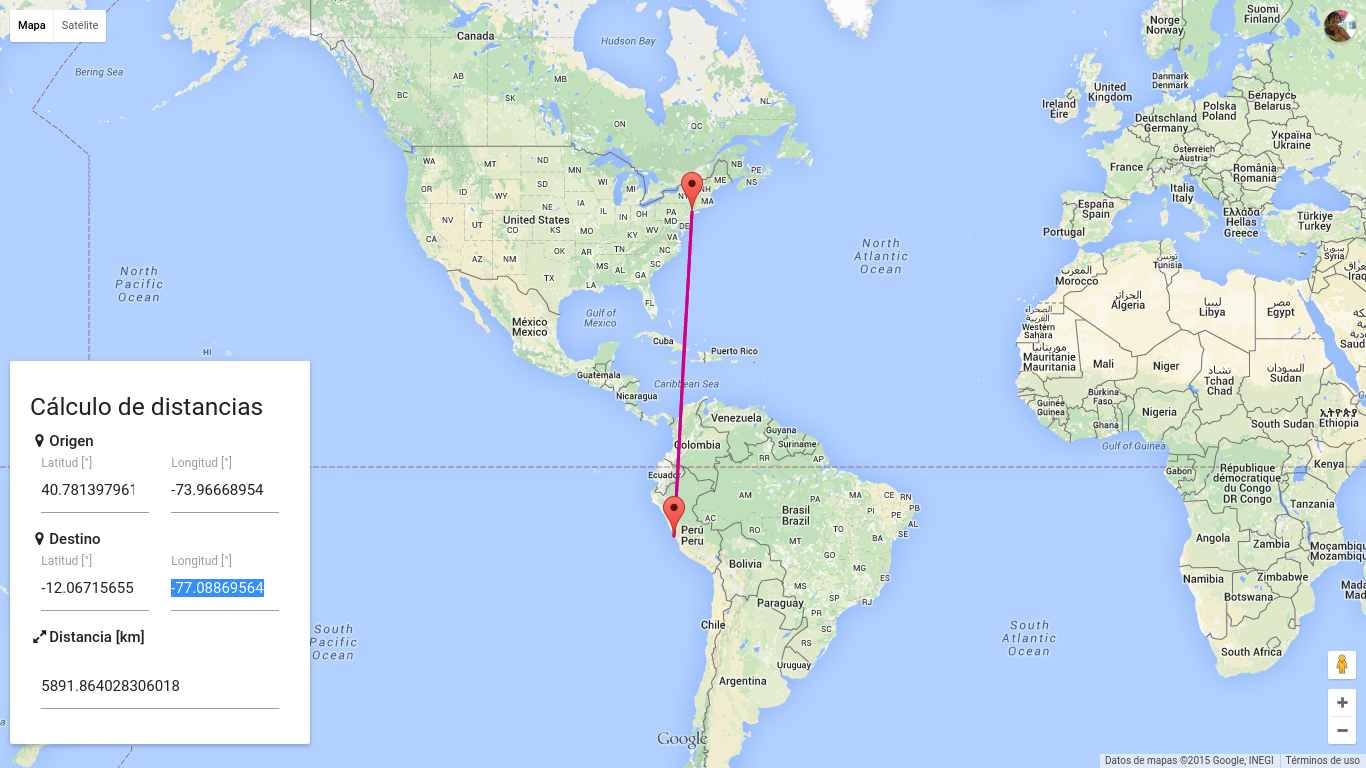
\includegraphics[width=\textwidth]{./laboratorio_1/problema04js_sample.png}
      \end{figure}

      \noindent Para las pruebas de este programa se tomaron las coordenadas de
      Central Park, Ney York, Estados Unidos y El Parque de las leyendas,
      Lima, Perú.
      \vspace{\fill}

  \newpage
  \subsection*{Problema 5}
    \noindent El día juliano es el número de orden que le corresponde a una
    fecha dada; por ejemplo, el 01 de enero sería el día juliano 1 y el 31
    de diciembre sería el día juliano 365. Hacer un programa para
    convertir de día juliano a fecha. ¿A que fecha corresponde el día
    juliano 220? Variar el programa para tener en cuenta los años
    bisiestos: múltiplos de 4, excepto los que terminen en 00, como el
    año 2000.

    \subsubsection*{Solución}
      \begin{listing}[H]
        \caption{Cálculo de la fecha juliana.}
        \label{script05}
        \inputminted[firstline=5,lastline=44]{matlab}{./laboratorio_1/problema05.m}
      \end{listing}
      \vspace{-1em}
      \noindent Continúa en la página siguiente.
      \vspace{\fill}

      \newpage
      \noindent Continuación del \emph{script} \ref{script05}.
      \begin{listing}[H]
        \inputminted[firstline=46]{javascript}{./laboratorio_1/problema05.m}
      \end{listing}

      \begin{listing}[H]
        \caption{Ejemplo de ejecución del programa mostrado en el
        \emph{script} \ref{script05}}
        \label{script05sample}
        \inputminted{text}{./laboratorio_1/problema05_sample.txt}
      \end{listing}

      \noindent La solución se planteó, considerando el día juliano como el
      número ordinal de la fecha correspondiente dentro de un año dado.
      \vspace{\fill}

  \newpage
  \subsection*{Problema 6}
    \noindent Se tiene un cuadrado de lado $L$ y una circunferencia inscrita
    en él. Supongamos que lanzamos pequeños dardos a gran distancia.
    Muchos caerán dentro y otros caerán fuera de la circunferencia. Sea
    $n$ el número de dardos que caen dentro del circulo y $N$ el número
    de dardos que caen dentro del cuadrado. La razón de estas dos
    cantidades será proporcional a la razón de las áreas del cuadrado y de
    la circunferencia. Hallar una aproximación de $\pi$ en función de $n$
    y $N$. Hacer un programa para hallar el valor de $\pi$ para un valor
    de $N$ introducido por el usuario.

    \subsubsection*{Solución}
      \begin{listing}[H]
        \caption{Cálculo de aproximado de $\pi$}
        \label{script06}
        \inputminted[firstline=5]{matlab}{./laboratorio_1/problema06.m}
      \end{listing}

      \begin{listing}[H]
        \caption{Ejemplo de ejecución del programa mostrado en el
        \emph{script} \ref{script06}}
        \label{script06sample}
        \inputminted{text}{./laboratorio_1/problema06_sample.txt}
      \end{listing}
      \vspace{\fill}

  \newpage
  \subsection*{Problema 7}
    \noindent Hacer una gráfica en 3 dimensiones de la curva gaussiana:
    %$$z=A\cdot\mathrm{e}^{\right( x^2 + y^2 \left)}$$
    $$z = A \cdot \mathrm{e}^{\left(x^2 + y^2\right)}$$
    donde $A=10$ es la amplitud de la curva. Utilice una grilla para el
    dominio: $-10 < x < 10\ \wedge\ -10 < y < 10$

    \begin{enumerate}
      \item Considere que la dimensión de la grilla es unitaria.
      \item Considere que la dimensión de la grilla es 0.2.
      \item Modifique el programa para visualizar curvas de nivel.
    \end{enumerate}

    \subsubsection*{Solución}
      \begin{listing}[H]
        \caption{Programa para graficar la función $z = A \cdot \mathrm{e}^{\left(x^2 + y^2\right)}$}
        \label{script07}
        \inputminted[firstline=5]{matlab}{./laboratorio_1/problema07.m}
      \end{listing}

      \begin{listing}[H]
        \caption{Ejemplo de ejecución del programa mostrado en el
        \emph{script} \ref{script07}}
        \label{script07sample}
        \inputminted{text}{./laboratorio_1/problema07_sample.txt}
      \end{listing}

      \begin{figure}[H]
        \caption{Resultados de la ejecucion del \emph{script} \ref{script07}.}
        \label{script07figure1}
        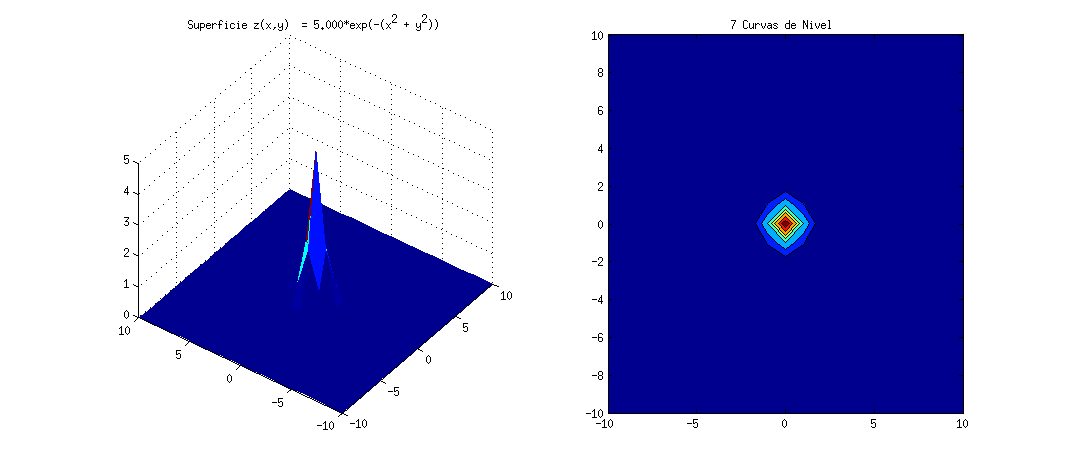
\includegraphics[width=\textwidth]{./laboratorio_1/problema07_sample1.png}
        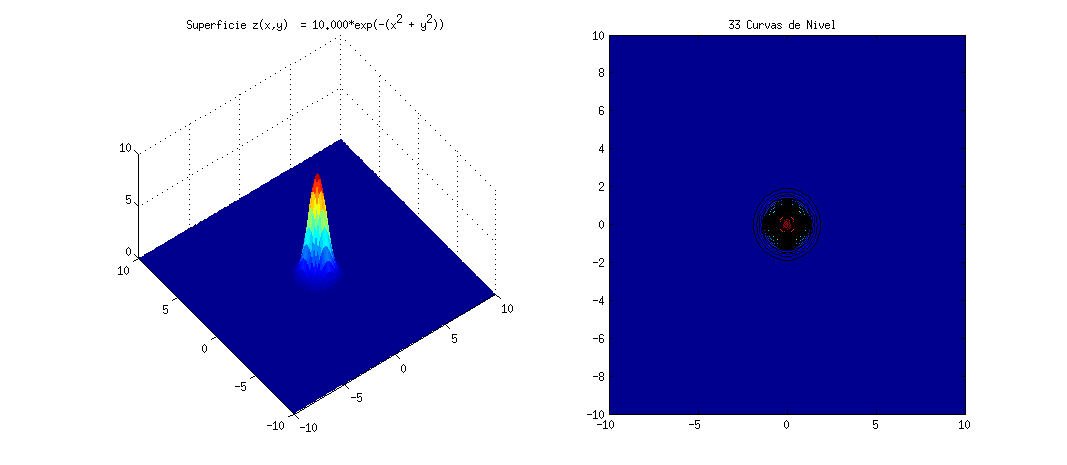
\includegraphics[width=\textwidth]{./laboratorio_1/problema07_sample2.png}
      \end{figure}

\end{document}
